\section{Discussion}
We  note at the outset that the sensitivity analysis investigates the numerical model rather than the physiological one. However, since the numerical model has been validated with experimental data  \cite{Dormanns2015,Mathias2018},  the results indicate parameters (and therefore areas) of importance for physiologists and modellers. The integration times $t_1,t_2$ are the start and end of neuronal stimulation. Decreasing or increasing these time does not significantly alter the ranking of the parameters. We discuss below results for each QoI individually. 


\subsection{Average ECS Potassium}
It is interesting to note for this particular quantity of interest that the first and third most important parameters are associated not with a \pot channel but the persistent \na channel, NaP.  The neuron model used in this analysis was developed from the work of Kager et al \cite{Kager2000a} and Chang et al \cite{Chang2013}.
The differential equation governing $m_4$,  the activation variable for the NaP channel, is given by equation (\ref{eqn:m4}).
%\begin{eqnarray}
%\frac{d m_4}{dt} = m_{4 \alpha}(1 - m_4) - (m_{4\beta} \, m_4), \label{eqn:m4alpha} \nonumber \\
%m_{4 \alpha}= \frac{1}{6(1 + \exp(-((c_1 v_d) + c_2)))} \nonumber \\
%m_{4 \beta} = m4_{\alpha} \exp(-((c_1 v_d) + c_2))
%\end{eqnarray}.

The inactivation of the NaP channel is very small compared to activation and therefore these parameters make little impact on the extracellular \pot. 
Scatter plots for the average of \pot in the  ECS against the parameters $\theta_{61}$ and $\theta_{62}$ are shown in Figure \ref{fig:scatter}.  For each parameter, there is a linear trend where increasing the parameter yields either an increase or decrease in the \pot ECS. The characteristic time for the activation variable for the NaP channel is defined as $\tau=\frac{1}{m_{4 \alpha}+m_{4 \beta}}$ which, by using equation (\ref{eqn:m4}), is constant (6 ms). The scatter plots also indicate this definition. These results show that a variation of $\pm 10 \%$ in either $\theta_{62}$ or $\theta_{63}$ can either reduce or increase the extracellular \pot  by approximately $15 \%$. We should note that these results do not take into account the spatial buffering carried out by the astrocytic syncytium which may have a significantly greater effect on the extracellular \pot \cite{Bellot-Saez2017,Kenny2018b}. 

\begin{figure}
\centering
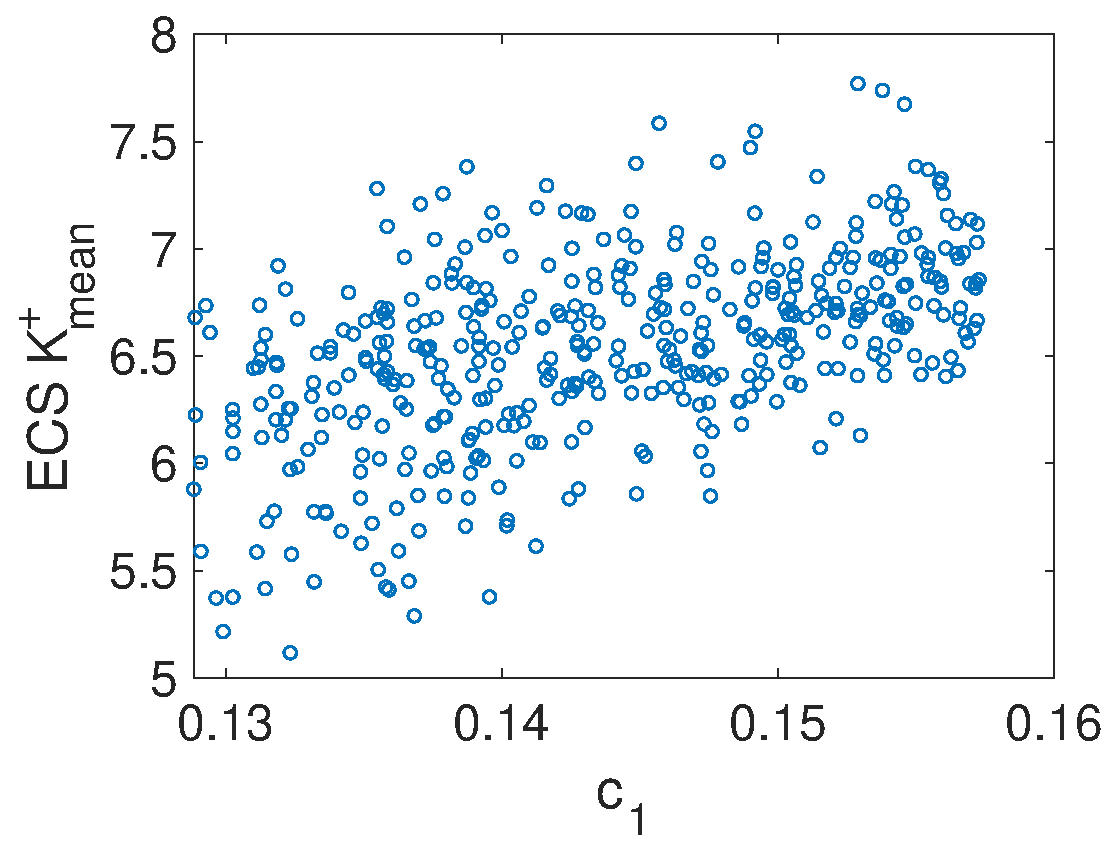
\includegraphics[width=0.49\linewidth]{Figures/Scatter_62_K_ECS}
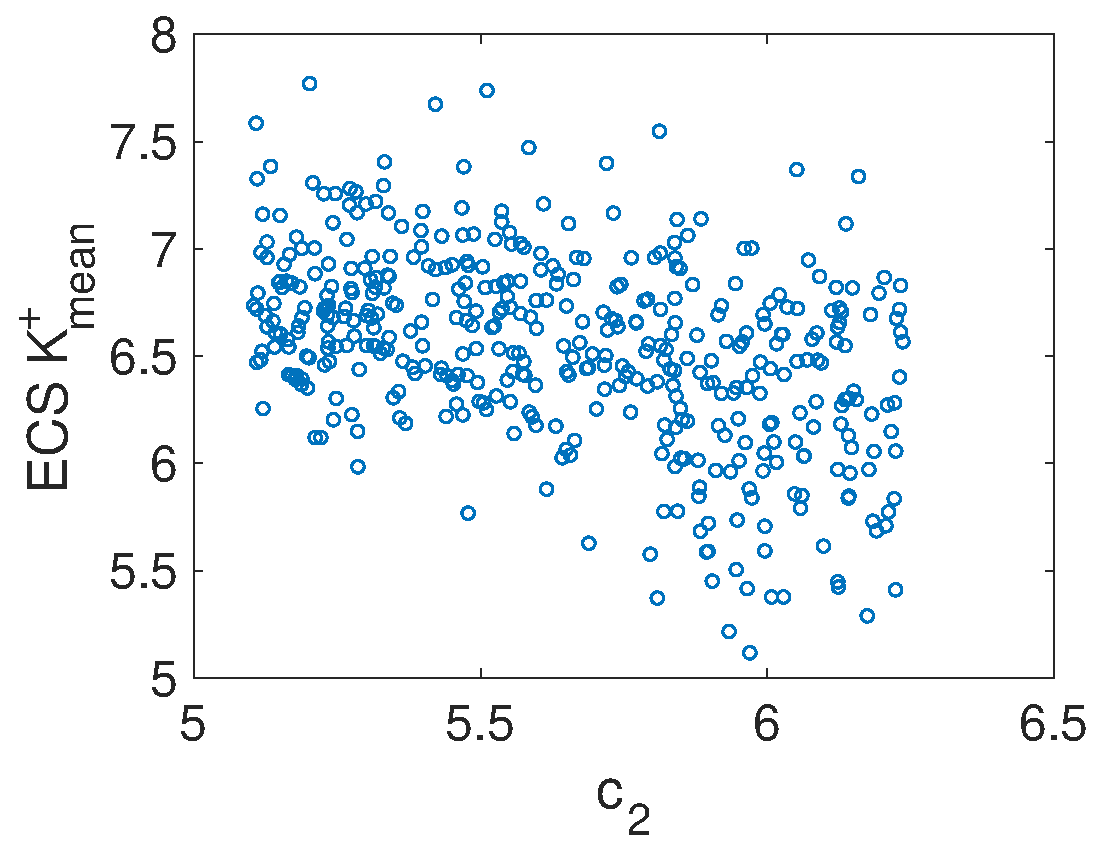
\includegraphics[width=0.48\linewidth]{Figures/Scatter_63_K_ECS}
\caption{Left: scatter plot of $\theta_{62}$ and the average ECS potassium \eqref{K_ECS_Mean}; right: scatter plot of $\theta_{63}$ and the average ECS potassium \eqref{K_ECS_Mean}.}
\label{fig:scatter}
\end{figure}
The main driver for \pot in the extracellular space is the \pot \na ATP-ase pump which has the general form given by (in the dendrite)  
\begin{eqnarray}\label{eqn:ATP-ase}
\frac{(Na^{+}_{d})^3}{\left( Na^{+}_{d}+Na^{+}_{d,baseline}\right)^3}\frac{(K^{+}_e)^{2}}{\left( K^+_e +K^+_{e,baseline}\right) ^2}.
\end{eqnarray}
The ATP-ase pumps out \na and in \pot in the ratio of 3 to 2, hence the \na in the dentrite has a large effect on the extracellular \pot as seen in equation (\ref{eqn:ATP-ase}) and strengthens the result that the NaP channel has the most effect on the \pot. One could have expected the NaT (transient \na) channel to be prominent however, it has a fast inactivation variable and, although it produces a larger flux, does so over a shorter time.  
\subsection{Average Volumetric Flow Rate}
In the presented model, the main pathway for neurovascular coupling is that of the \pot pathway. Here the astrocyte takes up \pot ~from the synaptic cleft and provides an efflux into the perivascular space (PVS) via the BK channel. The smooth muscle cell detects this increase in PVS \pot and through the inwardly rectifying channel, $K_{IR}$, hypopolarises the SMC, shutting off the voltage mediated \ca channel.  \ca is therefore reduced and the SMC dilates. As stated in the Section~\ref{sec:results}, the most important parameter is the shift parameter $\theta_{141}$ in the $K_{IR}$ conductance \eqref{eqn:gkir} determining the magnitude of ion flux per unit change in the membrane potential away from the equilibrium (Nernst potential).  Compared to the other parameters defining the $K_{IR}$ conductance, $\theta_{141}$ is large with a nominal value of 12.6 whereas $\theta_{140}=4.2 \times 10^{-4} \mu M^{-1}$ and $\theta_{142} = -7.4 \times10^{-2} mV^{-1}$. Hence, for constant membrane potential and \pot,   variations in $\theta_{141}$ produce exponentially large variations in the $K_{IR}$ channel conductance allowing substantial efflux of \ca from the SMC and a dilation of the vessel $\left(\frac{dR}{dt}> 0\right)$. \\

The second most important parameter is the power index for the cytosolic SMC \ca which mediates the four state latch model of Hai and Murphy \cite{Hai1988} that is used in this model, in particular the rate of phosphorylation of  myosin and the actin-myosin complex.  Variations in \ca as predominantly dictated by the $K_{IR}$ channel will therefore have a direct effect on the dilation/contraction properties of the SMC and hence the perfusing vessel radius.  
The remaining three parameters have significantly lower total Sobol' indices and therefore only make small contributions to the QoI.
 
\subsection{$[AM+AM_p]_{min}$}
We see similar parameters appearing as most important for this QoI and the average volumetric flow rate QoI, which is to be expected given the strong relationship between the radius dilation/contraction phenomenon and the total quantity of actin/myosin complex and its phosphorylated compliment. In fact, this QoI serves as a test of the statistical mechanism in that the only two non-repeating parameters (in the list of five most important) between the volumetric flow rate QoI and the actin/myson complex QoI are $\theta_{120}$ and $\theta_{136}$, which, as noted above, are significantly less import than the leading parameters.
%\subsection{Other QoIs analysed}
%
%The methodology was tested on a number of other QoIs that are not reported above. Each QoI, listed below, was not reported for one of three reasons: (i) the analysis failed because the QoI was too nonlinear, (ii) the QoI was nearly constant and did not warrant global sensitivity analysis, or (iii) the results were very similar to results reported in the article.
%
%\subsubsection{Time lag from when the stimulus was applied until the state $AM_p$ attained its minimum}
%For this QoI, the linear surrogate had a relative $L^2$ error of 59\%. Hence our screening step could not be performed so the analysis failed. 
%%\todo[inline]{Tim: can we supply a reason for this failure as well as that below? Joey: Its hard to say anything too precise without getting into a lot of hairy details. We can say something somewhat generally about the difference in averages, minimums, and time lags.}
%
%\subsubsection{Time lag from when the stimulus was applied until the radius attained its maximum} 
%For this QoI, the linear surrogate had a relative $L^2$ error of 47\%. As in the previous QoI, the screening step could not be performed so the analysis failed. 
%
%\subsubsection{Maximum potassium concentration in the Astrocyte}
%This QoI was approximately constant as the parameters varied.
%
%\subsubsection{Average potassium concentration in the Astrocyte}
%This QoI was approximately constant as the parameters varied.
%
%
